% cordillera-climate.tex
% ----------------------------------------------------------------------

% Copernicus manuscript
\documentclass[tc, ms]{copernicus}

% Copernicus final print
%\documentclass[tc]{copernicus}

% Copernicus discussion paper
%\documentclass[tcd, hvmath]{copernicus_discussions}

% Copernicus-like latex2rtf compatible
%% copernicus_rtf.tex
% ------------------

% Base class and packages
\documentclass{article}
\usepackage{color}
\usepackage{geometry}
\usepackage{graphicx}
\usepackage{setspace}
\onehalfspacing

% Replacements for bibtex commands
\newcommand{\citep}[1]{(\textcolor{blue}{#1})}
\newcommand{\citet}[1]{\textcolor{blue}{#1}}

% Replacements for Copernicus commands
\newcommand{\introduction}[0]{\section{Introduction}}
\newcommand{\conclusions}[0]{\section{Conclusions}}
\newcommand{\tophline}[0]{\hline}
\newcommand{\middlehline}[0]{\hline}
\newcommand{\bottomhline}[0]{\hline}
\newcommand{\unit}[1]{\ensuremath{\mathrm{#1}}}
\newcommand{\degree}[0]{\ensuremath{^{\circ}}}

% Ignore other Copernicus commands
\newcommand{\runningtitle}[1]{}
\newcommand{\runningauthor}[1]{}
\newcommand{\received}[1]{}
\newcommand{\correspondence}[1]{}
\newcommand{\pubdiscuss}[1]{}
\newcommand{\revised}[1]{}
\newcommand{\accepted}[1]{}
\newcommand{\published}[1]{}



% Coloured hyperlinks
\usepackage[colorlinks]{hyperref}

% Encoding
\usepackage[T1]{fontenc}

% Figure directory
\graphicspath{{figures/}}

% ----------------------------------------------------------------------
\begin{document}\hack{\sloppy}
% ----------------------------------------------------------------------

% Title
\title{Numerical simulation of the Cordilleran ice sheet through the last glacial cycle}

% Authors
\author[1,2]{J.~Seguinot}
\runningauthor{J.~Seguinot et~al.}
\correspondence{J.~Seguinot (julien.seguinot@natgeo.su.se)}

% Running title
\runningtitle{Climate forcing for Cordilleran ice sheet simulations}

% Affiliations
\affil[1]{Department of Physical Geography and Quaternary Geology and the Bolin Centre for Climate Research, Stockholm University, Stockholm, Sweden}
\affil[2]{Helmholtz Centre Potsdam, GFZ German Research Centre for Geosciences, Potsdam, Germany}

% For Copernicus
\received{}
\accepted{}
\published{}

% Title
\firstpage{1}
\maketitle

% Abstract
\begin{abstract}
\end{abstract}


% ----------------------------------------------------------------------
\introduction
\label{sec:intro}
% ----------------------------------------------------------------------


% ----------------------------------------------------------------------
\section{Model setup}
\label{sec:model}
% ----------------------------------------------------------------------


% ----------------------------------------------------------------------
\section{Results}
\label{sec:results}
% ----------------------------------------------------------------------


% ----------------------------------------------------------------------
\section{Discussion}
\label{sec:discussion}
% ----------------------------------------------------------------------


% ----------------------------------------------------------------------
\conclusions
\label{sec:concl}
% ----------------------------------------------------------------------

% Acknowledgements
%\begin{acknowledgements}
  % Author contributions
  %\hack{\noindent}\textit{Author contributions.}
%\end{acknowledgements}

% References
%\input{references.bbl}
%\newpage

% ----------------------------------------------------------------------
% Floats
% ----------------------------------------------------------------------

% fig:locmap
%\begin{figure}
%  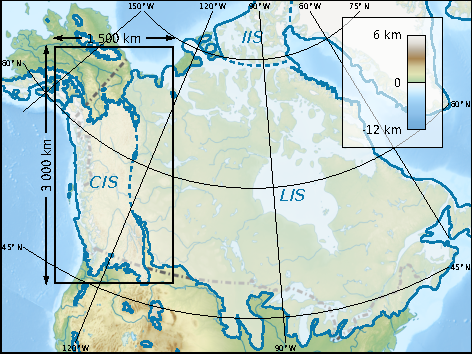
\includegraphics{cordillera-climate-locmap}
%  \caption{}
%  \label{fig:locmap}
%\end{figure}

% ----------------------------------------------------------------------
\end{document}
\endinput
% ----------------------------------------------------------------------
